% Classes of src/gui (CapGui) and their dependencies. Paper: section "CapGui" (fig:gui); Doxygen: CapGui.hpp.
%   pdflatex GuiClasses.tex; pdftoppm -r 200 -png -singlefile GuiClasses.pdf GuiClasses;
%   pdftocairo -svg GuiClasses.pdf GuiClasses.svg
\documentclass[tikz,border=2pt]{standalone}
% Shared style of the class diagrams of CAP (figures/*Classes.tex): \input after \documentclass[tikz]{standalone}.
%  - boxes: blue = abstract base class, light blue = class, green = entry class of the folder (steering class, task),
%    yellow = free functions (tools), grey = class of another folder;
%  - arrows: open triangle = inherits from; dashed with diamond = owns (holds); dashed with arrow = uses.
\usepackage[scaled=0.92]{helvet}
\usetikzlibrary{arrows.meta,shapes.multipart,positioning,fit,backgrounds,calc}
\renewcommand{\familydefault}{\sfdefault}
\definecolor{abstract}{HTML}{D6E4F5}
\definecolor{concrete}{HTML}{EEF4FB}
\definecolor{steer}{HTML}{DCEFD9}
\definecolor{tools}{HTML}{FFF8E6}
\definecolor{external}{HTML}{E9E9E9}
\definecolor{dependline}{HTML}{8A6D3B}
\definecolor{folder}{HTML}{F7F7F7}
\tikzset{
  every picture/.style={font=\scriptsize},
  cls/.style={draw, fill=concrete, align=center, inner sep=2.5pt, text width=#1, font=\tiny},
  cls/.default=3.0cm,
  abs/.style={cls=#1, fill=abstract},
  abs/.default=3.0cm,
  steer/.style={cls=#1, fill=steer, line width=0.8pt},
  steer/.default=4.2cm,
  tool/.style={cls=#1, fill=tools},
  tool/.default=4.2cm,
  ext/.style={cls=#1, fill=external, dashed},
  ext/.default=2.6cm,
  fam/.style={draw, rectangle split, rectangle split parts=2, rectangle split part fill={#1,white},
              rectangle split part align={center,left}, inner sep=2.5pt, align=left},
  inherit/.style={-{Triangle[open,length=2.2mm,width=2.2mm]}, thin},
  uses/.style={dashed, dependline, -{Stealth[length=1.6mm]}, thin},
  owns/.style={dashed, dependline, {Diamond[length=2.4mm,width=1.6mm]}-, thin},
  lbl/.style={font=\tiny, text=dependline, align=center},
  note/.style={font=\tiny, align=left, text=black!70},
  title/.style={font=\footnotesize\bfseries, anchor=north west},
}
% a member line in a class box
\newcommand{\m}[1]{\\#1}
\newcommand{\cn}[1]{{\scriptsize\textbf{#1}}}
\newcommand{\an}[1]{{\scriptsize\textbf{\textit{#1}}}}

% legend common to the class diagrams (place with \legendat{x}{y})
\newcommand{\legendat}[2]{%
  \begin{scope}[shift={(#1,#2)}, font=\tiny]
    \node[abs=0.9cm, minimum height=3mm, inner sep=1pt] (lA) at (0,0) {abstract};
    \node[cls=0.9cm, minimum height=3mm, inner sep=1pt, right=1mm of lA] (lC) {class};
    \node[steer=1.1cm, minimum height=3mm, inner sep=1pt, right=1mm of lC] (lS) {entry class};
    \node[tool=1.1cm, minimum height=3mm, inner sep=1pt, right=1mm of lS] (lT) {functions};
    \node[ext=1.3cm, minimum height=3mm, inner sep=1pt, right=1mm of lT] (lE) {other folder};
    \draw[inherit] ($(lE.east)+(1mm,0)$) -- ++(5mm,0) node[right, inner sep=1pt] (l1) {inherits};
    \draw[owns] ($(l1.east)+(1mm,0)$) -- ++(5mm,0) node[right, inner sep=1pt] (l2) {owns};
    \draw[uses] ($(l2.east)+(1mm,0)$) -- ++(5mm,0) node[right, inner sep=1pt] {uses};
  \end{scope}}

\begin{document}
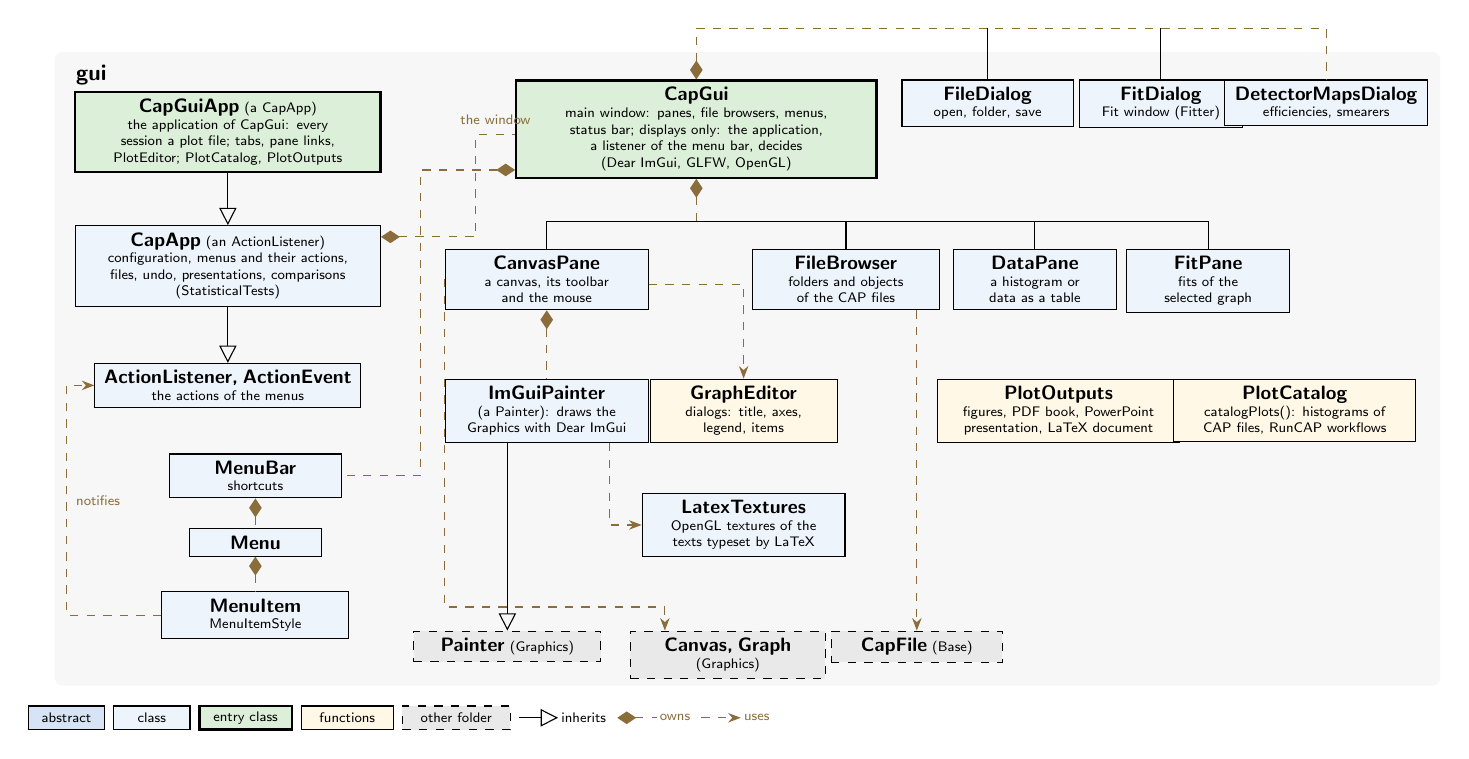
\begin{tikzpicture}[every node/.append style={anchor=north}]
  \begin{scope}[on background layer]
    \fill[folder, rounded corners=3pt] (-0.15,-0.25) rectangle (17.45,-8.3);
  \end{scope}
  \node[title] at (0.0,-0.3) {gui};

  % application (left column)
  \node[steer=3.7cm] (GuiApp) at (2.05,-0.75)
    {\cn{CapGuiApp} \tiny(a CapApp)\m{the application of CapGui: every}\m{session a plot file; tabs, pane links,}\m{PlotEditor; PlotCatalog, PlotOutputs}};
  \node[cls=3.7cm] (App) at (2.05,-2.45)
    {\cn{CapApp} \tiny(an ActionListener)\m{configuration, menus and their actions,}\m{files, undo, presentations, comparisons}\m{(StatisticalTests)}};
  \node[cls=3.2cm] (Action) at (2.05,-4.2) {\cn{ActionListener, ActionEvent}\m{the actions of the menus}};
  \node[cls=2.0cm] (MenuBar) at (2.4,-5.35) {\cn{MenuBar}\m{shortcuts}};
  \node[cls=1.5cm] (Menu) at (2.4,-6.3) {\cn{Menu}};
  \node[cls=2.2cm] (MenuItem) at (2.4,-7.1) {\cn{MenuItem}\m{MenuItemStyle}};
  \draw[inherit] (GuiApp.south) -- (App.north);
  \draw[inherit] (App.south) -- (Action.north);
  \draw[owns] (MenuBar.south) -- (Menu.north);
  \draw[owns] (Menu.south) -- (MenuItem.north);
  \draw[uses] (MenuItem.west) -- (0.0,0 |- MenuItem.west) |- node[lbl, pos=0.25, right]{notifies} (Action.west);

  % window
  \node[steer=4.4cm] (Gui) at (8.0,-0.6)
    {\cn{CapGui}\m{main window: panes, file browsers, menus,}\m{status bar; displays only: the application,}\m{a listener of the menu bar, decides}\m{(Dear ImGui, GLFW, OpenGL)}};
  \draw[owns] (App.east |- 0,-2.6) -- (5.2,-2.6) |- node[lbl, pos=0.75, above]{the window} (Gui.west |- 0,-1.3);
  \draw[owns] (Gui.west |- 0,-1.75) -- (4.5,-1.75) |- (MenuBar.east);

  \node[cls=2.0cm] (FileDialog) at (11.7,-0.6) {\cn{FileDialog}\m{open, folder, save}};
  \node[cls=1.9cm] (FitDialog) at (13.9,-0.6) {\cn{FitDialog}\m{Fit window (Fitter)}};
  \node[cls=2.4cm] (Maps) at (16.0,-0.6) {\cn{DetectorMapsDialog}\m{efficiencies, smearers}};
  \draw[owns] (Gui.north) -- (8.0,0.05) -- (16.0,0.05) -- (Maps.north);
  \draw (FileDialog.north) -- (11.7,0.05);
  \draw (FitDialog.north) -- (13.9,0.05);

  \node[cls=2.4cm] (Canvas) at (6.1,-2.75) {\cn{CanvasPane}\m{a canvas, its toolbar}\m{and the mouse}};
  \node[cls=2.2cm] (Browser) at (9.9,-2.75) {\cn{FileBrowser}\m{folders and objects}\m{of the CAP files}};
  \node[cls=1.9cm] (DataPane) at (12.3,-2.75) {\cn{DataPane}\m{a histogram or}\m{data as a table}};
  \node[cls=1.9cm] (FitPane) at (14.5,-2.75) {\cn{FitPane}\m{fits of the}\m{selected graph}};
  \draw[owns] (Gui.south) -- (8.0,-2.4);
  \draw (6.1,-2.4) -- (14.5,-2.4);
  \foreach \c in {Canvas, Browser, DataPane, FitPane} \draw (\c.north |- 0,-2.4) -- (\c.north);

  % drawing
  \node[cls=2.4cm] (Painter) at (6.1,-4.4) {\cn{ImGuiPainter}\m{(a Painter): draws the}\m{Graphics with Dear ImGui}};
  \node[tool=2.2cm] (Editor) at (8.6,-4.4) {\cn{GraphEditor}\m{dialogs: title, axes,}\m{legend, items}};
  \node[cls=2.4cm] (Tex) at (8.6,-5.85) {\cn{LatexTextures}\m{OpenGL textures of the}\m{texts typeset by LaTeX}};
  \draw[owns] (Canvas.south) -- (Painter.north);
  \draw[uses] (Canvas.east |- 0,-3.2) -| (Editor.north);
  \draw[uses] (6.9,0 |- Painter.south) |- (Tex.west);

  \node[tool=2.9cm] (Outputs) at (12.6,-4.4) {\cn{PlotOutputs}\m{figures, PDF book, PowerPoint}\m{presentation, LaTeX document}};
  \node[tool=2.9cm] (Catalog) at (15.6,-4.4) {\cn{PlotCatalog}\m{catalogPlots(): histograms of}\m{CAP files, RunCAP workflows}};

  % other folders
  \node[ext=2.2cm] (GPainter) at (5.6,-7.6) {\an{Painter} \tiny(Graphics)};
  \node[ext=2.3cm] (GCanvas) at (8.4,-7.6) {\cn{Canvas, Graph}\m{(Graphics)}};
  \node[ext=2.0cm] (CapFile) at (10.8,-7.6) {\cn{CapFile} \tiny(Base)};
  \draw[inherit] (5.6,0 |- Painter.south) -- (GPainter.north);
  \draw[uses] (Canvas.west) -- (4.8,0 |- Canvas.west) |- (7.6,-7.3) -- (7.6,0 |- GCanvas.north);
  \draw[uses] (10.8,0 |- Browser.south) -- (CapFile.north);
  \legendat{0.0}{-8.55}
\end{tikzpicture}
\end{document}
